\section{Evaluation and Discussion}
% \subsection{Regression Models} This needs to be moved to a previous section where we outline the regression side
% A variety of different regression models were trained and validated on the data each performing to a degree of competence, however a large margin of accuracy can be discovered when comparing the models together.


\subsection{NLP}
The sections covers chatbot's performance in natural language understanding, response accuracy, user experience, and technical robustness. 
\subsubsection{Natural Language Understanding (NLU)}
\begin{itemize}
    \item \textbf{Intent Recognition:} The chatbot correctly identifies user intentions, such as searching for train tickets, specifying travel date and time, querying about prices or requesting delay information or requesting for contingency plans in case of partial or full line blockage.
    \item \textbf{Entitiy Recognition:} The chatbot accurately identifies key entities like locations (departure and arrival), dates, times, and ticket preferences (e.g., on-way or return), blockage type etc.
    \item \textbf{Context Handling:} The chatbot is effective in maintaining context over a multi-turn conversation and understanding follow-up queries.
\end{itemize} 

\subsubsection{Response Accuracy}
\begin{itemize}
    \item \textbf{Correctness:} The chatbot accurately provided the information of the cheapest train ticket, delayed time display or alternate routes as per contingency plans.
    \item \textbf{Relevance:} The chatbot's responses are appropriate as per user queries.
    \item \textbf{Completeness:} The chatbot responses are comprehensive, providing all necessary information to the user.
\end{itemize} 

\subsubsection{User Experience (UX)}
\begin{itemize}
    \item \textbf{Ease of Use:} As per the usability testing in \ref{tab:usability_testing} carried out by different UEA students, the feedback was positive about chatbot being easy to use.
    \item \textbf{Response Time:} The response time of the answer was fairly short. The multi-processing implemented which runs the scraper scripts asynchronously instead of one by one, saved a lot of response time.
    \item \textbf{User Satisfaction:} The overall response from both of the UEA students who carried usability testing was positive and satisfactory.
\end{itemize} 

\subsubsection{Technical Robustness}
\begin{itemize}
    \item \textbf{Reliability:} The developed chatbot have consistence performance with correct / appropriate responses.
    \item \textbf{Error Handling:} The chatbot is robust enough to handle conversations related to different tasks as well as if there are mis-spelled words in the user's input or even there is partial information given.
    \item \textbf{Integration:} The integrity constraints were applied in the chatbot to prevent delivering invalid information to the users.
\end{itemize}

\subsubsection{Areas for Improvement \& Future Enhancements}
\textbf{Part A: Find cheapest train ticket}

\begin{itemize}
    \item In order to make the search for the cheapest train tickets more dynamic and accurate, the user should be allowed to enter other parameters, such as the number of adults and children and whether or not they have a rail card. If so, inquire about the kind of railcard, etc.
    \item The user should be able to request a return ticket all at once rather than having to wait for the one-way search to finish before responding to the chatbot's request to inquire whether they would also like a return ticket. The user may be able to save more money in this method.
    \item Even though multi-processing is used to run all of the scrapers asynchronously, the cheapest train fare search still takes a long time since the system needs time to render the response on the GUI. Redesigning the system could improve its performance.
\end{itemize}

\textbf{Part B: Find train delay}

\begin{itemize}
    \item 
    \item 
    \item 
\end{itemize}

\textbf{Part C: Fetch contingency plans}

\begin{itemize}
    \item Give the user the ability to request backup plans between any station on the Great Eastern track, not only the one between Colchester and Norwich.
    \item The system should be able to receive additional inputs based on various situations, such as whether the obstruction is the result of a natural disaster like heavy rain or flooding, and then return the contingency plans in accordance with those inputs in order to make the search more dynamic. Train services must be halted, etc., if the temperature rises beyond thirty degrees.
    \item It is also possible to give the backup plans due consideration. In the event of a blockage between two stations, the system ought to provide specific solutions, especially if it is close to midnight. A certain kind of response should be given if it's peak hour and so on.
\end{itemize}

\subsection{Regression Models}
The sections below outline and describe the research efforts made into regression models and the performance metrics of each.
% \subsubsection{Multi-layer Perceptron (MLP) Regressor}
% A simple MLP model was integrated using the

\paragraph{K Nearest Neighbors Regressor:} \label{Sec: KNN tuning}
The parameter which configured the number of neighbours of the K-Nearest Neighbors (KNN) regression model was manually tuned using a $for$ loop which iteratively increased the value of $k$ and scored the model accordingly using metrics outlines in Section \ref{Sec: Regression Metrics & performance}. Figure \ref{Fig: KNN K vs k} shows the iteration of $k$, the results of these $k$ values can be seen in Figures: \ref{Fig: KNN K vs MAE}, \ref{Fig: KNN K vs R^2}, \ref{Fig: KNN K vs RMSE}. From these results we can see minimal prediction accuracy improvement when $k > 30$, on the contrary we can see great improvements when $k$ is increased to 20. With these results in mind, a $k$ value of 50 was used to maximise potential accuracy as the trade off between prediction time per value of $k$ was minimal.

\paragraph{Random Forest Regressor:}
The Random Forest (RF) regression model was built with near-default parameters. The only specific change made to the configuration of the model was the number of estimators. Similar to the manual tuning of the KNN model outlined in Section \ref{Sec: KNN tuning}, an iterative $for$ loop was employed to score the model per number of estimators. Figure \ref{Fig: RF nn vs nn} displays the number of estimators searched, an initial value of 5 was chosen with an iterative increase of 1 until a value of 10 was selected. Once the value of estimators reached 10, an incrementation of 5 was chosen instead to increase efficiency. Table \ref{tab: RF score per K} displays scores per value of $k$. Figures \ref{Fig: RF MSE vs nn}, \ref{Fig: RF r^2 vs nn}, \ref{Fig: RF RMSE vs nn} show the models performance per iteration. From these results we can see the performance peaked at an estimator value of 8.
-
\begin{table}[!htbp]
    \centering
    % \begin{tabular}{|c|c|c|c|}
    \begin{tabularx}{\textwidth}{XXXX}
    \hline
    n\_estimators & RMSE & MAE & R2 \\
    \hline
    5 & 1692.184531 & 322.930468 & 0.993185 \\
    6 & 1692.829572 & 322.482591 & 0.993180 \\
    7 & 1689.592844 & 322.124198 & 0.993206 \\
    \textbf{8} & \textbf{1683.224923} & \textbf{321.827668} & \textbf{0.993257} \\
    9 & 1682.711353 & 321.882941 & 0.993261 \\
    10 & 1686.329066 & 322.128959 & 0.993232 \\
    ... & ... & ... & ... \\
    100 & 1685.108628 & 322.103318 & 0.993242 \\
    \hline
    % \end{tabular}
    \end{tabularx}
    \caption{Performance results of the Random Forest Regression model}
    \label{tab: RF score per K}
\end{table}

\paragraph{XGBoost Regression:}
Similar the to K Nearest Neighbors and Random Forest models, the XGBoost model was implemented with default parameters with iteratively increasing number of estimators. Table \ref{tab:XGBoost score per N_estimators} and Figure \ref{fig: XGBoost estimators vs results} show the performance of the model per number of estimators. From these results we can see a correlation between an increased value of estimators and the models improved performance.


\begin{table}[h]
    \centering
    % \begin{tabular}{|c|c|c|c|}
    \begin{tabularx}{\textwidth}{XXXX}
    \hline
    \textbf{n\_estimators} & \textbf{RMSE} & \textbf{MAE} & \textbf{R2} \\
    \hline
    1 & 14423.881550 & 11689.875945 & 0.504871 \\
    2 & 10194.480707 & 8214.249700 & 0.752666 \\
    3 & 7270.192730 & 5782.620130 & 0.874210 \\
    4 & 5271.073107 & 4084.681260 & 0.933877 \\
    5 & 3932.805430 & 2900.675047 & 0.963191 \\
    ...&...&...&...\\
    % 6 & 3064.765834 & 2075.270793 & 0.977646 \\
    % 7 & 2530.248765 & 1506.208446 & 0.984764 \\
    % 8 & 2219.225104 & 1115.703541 & 0.988279 \\
    % 9 & 2047.260012 & 852.227672 & 0.990025 \\
    % 10 & 1955.658498 & 677.491905 & 0.990898 \\
    % 15 & 1861.595469 & 424.721672 & 0.991752 \\
    % 20 & 1848.114642 & 405.720689 & 0.991871 \\
    % 25 & 1833.428678 & 401.357044 & 0.992000 \\
    % 30 & 1814.992326 & 399.066723 & 0.992160 \\
    % 35 & 1801.847733 & 397.325036 & 0.992273 \\
    % 40 & 1783.585265 & 395.618465 & 0.992429 \\
    % 45 & 1775.365191 & 393.974004 & 0.992499 \\
    50 & 1770.881199 & 392.856774 & 0.992537 \\
    55 & 1766.922512 & 391.254378 & 0.992570 \\
    65 & 1752.241861 & 388.335768 & 0.992693 \\
    75 & 1740.280743 & 385.322977 & 0.992792 \\
    85 & 1733.922944 & 383.150441 & 0.992845 \\
    95 & \textbf{1728.680439} & \textbf{381.605032} & \textbf{0.992888} \\
    \hline
    % \end{tabular}
    \end{tabularx}
    \caption{Performance metrics for XGBoost regressor per value of n\_estimators}
    \label{tab:XGBoost score per N_estimators}
\end{table}

\paragraph{Metrics and results:}\label{sec: Metrics and results}
Table \ref{tab:model metrics} and Figures \ref{Fig: all_MAE}-\ref{Fig: all_RMSE} outline each models performance using the metrics described in Section. For a secondary evaluation, previous journey arrival and departure times were extracted from an online resource \href{https://www.recenttraintimes.co.uk/}{``Recent Train Times''} to be used as new unseen data. Figure \ref{fig: real delayed train times} and \ref{fig: real on-time train times} are two examples of the ground truth values extracted from the online source. Figure \ref{fig: inline_Regression models prediction of arrival time at Norwich} and \ref{fig: Regression model predicted arrival time at Norwich from London Liverpool Street} show the highest attaining classifiers predictions of the arrival time at Norwich using the data extracted.

\begin{table}[hbt!]
    \centering
    \begin{tabularx}{\textwidth}{XXXXX}
    \hline
    \textbf{Model Name} & \textbf{R2 Score} & \textbf{Mean Absolute Error} & \textbf{Root Mean Squared Error} & \textbf{Mean Squared Error} \\ 
    \hline
    MLP Regressor & 0.45369 & 7876.414635 & 15151.049907 & 229554313.277678 \\
    KN Regressor & 0.992975 & 337.436982 & 1718.046845 & 2951684.960503 \\
    XGB Regressor & 0.992888 & 381.605032 & 1728.680439 & 2988336.06081 \\
    RandomForest & \textbf{0.993242} & \textbf{322.103318} & \textbf{1685.108628} & \textbf{2839591.088781} \\
    Linear Regression & 0.394573 & 8650.629986 & 15949.750001 & 254394525.082963 \\
    Huber Regressor & 0.222805 & 5853.991688 & 18071.2504 & 326570091.003966 \\
    Lasso & 0.394573 & 8650.630322 & 15949.749997 & 254394524.969961 \\
    \hline
    \end{tabularx}
    \caption{Each model paired with the metric results}
    \label{tab:model metrics}
\end{table}

\begin{figure}[hbt!]
    \centering
    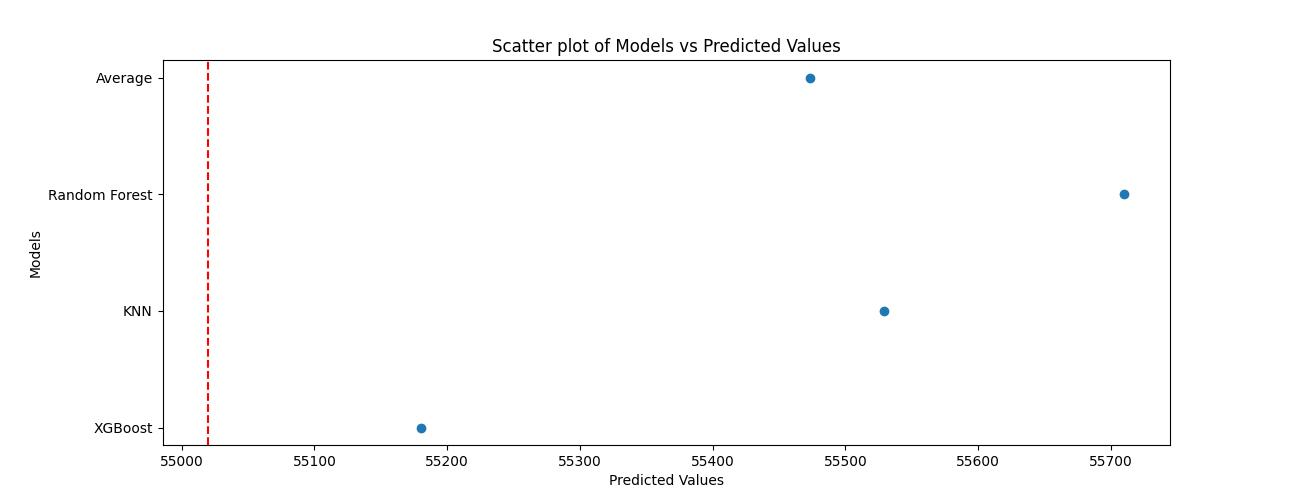
\includegraphics[width=\textwidth]{../regression_model/plots/Comparison/Scatter plot of Models vs Predicted Value 55020.jpeg}
    \caption[regression model predictions of previous journeys]{Regression models prediction of arrival time at Norwich from a departure from London Liverpool Station if delayed at Ipswich. The red dotted vertical line is ground truth.}
    \label{fig: inline_Regression models prediction of arrival time at Norwich}
\end{figure}

\paragraph{Model Evaluation:}
From the results described in Section \ref{sec: Metrics and results} Random Forest, K Nearest Neighbors and XGBoost regressor models appear superior. However, as shown in Figures \ref{fig: inline_Regression models prediction of arrival time at Norwich} and \ref{fig: Regression model predicted arrival time at Norwich from London Liverpool Street} each model will have a degree of inaccuracy when making predictions, as a result no single model would be a better choice for deployment. An average value was instead used to capture the accuracy of each model.
